\documentclass[html]{report}    % Specifies the document style.
\usepackage{graphicx}
\usepackage{verbatim}
\usepackage{tabularx}
\usepackage{marginnote}
%\usepackage[top=1.5cm, bottom=1.5cm, outer=5cm, inner=2cm, heightrounded, marginparwidth=2.5cm, marginparsep=2cm]{geometry}
\usepackage{amsmath}  % allows to use some of math functions
\usepackage{breqn}    % breaks equations in parts when needed
                           % The preamble begins here. 
\title{Multi-Agent Systems Project}  % Declares the document's title. 
\author{Panagiotis Chatzichristodoulou and Kirill Tumanov} 
%\date{November 29,2013}   % Deleting this command produces today's date.

\begin{document}           % End of preamble and beginning of text.

\maketitle                 % Produces the title.
\section{Introduction}
\subsection{Abstract}
This paper addresses the implementation of an intelligent negotiation agent. Furthermore, it discusses and analyses the results obtained from the experiments that were performed. 
Agent was developed based on the \textit{Genius} software platform, released by Delft University in 2009, in accordance with the \textit{ANAC'2013} guidelines and within the \textit{BOA} (Bidding Strategy, Opponent Model, Acceptance Strategy) framework. are based on the negotiation platform \textit{Genius}~\cite{genius}. It introduces an environment where agents can negotiate within different domains - discrete or continuous. Genius is the standard in the agent negotiation domain platform. The work was performed as a practical part of the Multi-agent Systems course at Maastricht University. 

\subsection{Framework}
Agents in the Genius platform can either be standalone, or belonging to the BOA framework. A single-entity agent can include all the required modules in itself or use the BOA components instead. Some additional helper classes can exist outside of the main agent class. A BOA agent implements the four needed models independently, and that makes it agent more versatile and extendable, due to its modular architecture. The Fig.~\ref{ANAC BOA} depicts how the BOA components are integrated.
\begin{figure}[htbp]
	  \caption{Scheme of a BOA framework}
	  \centering
	    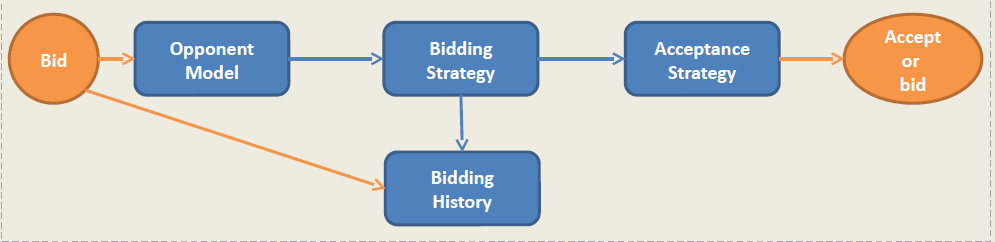
\includegraphics[width=1\textwidth]{fourmodels}
	  \label{ANAC BOA}
\end{figure}

\subsection{Agent summary}
The agent described in this paper was named NegoAgent. It behaves as a self-interested negotiator, meaning that it seeks to maximize its utility without taking into account the opponent's score, or the social welfare. However, it takes into account the discount factor $\delta$, and keeps track of the negotiation time in order to receive the highest utility possible. The agent is not going to accept not reasonable offers - it believes that "no deal is better than a bad deal", but when possible it tries to achieve a "win-win" compromise with an opponent. Overall, the agent is not tied to any specific domain or opponent behavior type, on contrary it tries to be adaptive to these challenges to its benefit.

A description of the BOA components used for agent development is given in subsequent sections, followed by modeling results and discussion.

\section{Bids Offering Strategy}
Agent's bid offering strategy was implemented as time-dependent (TD). The NegoAgent\_TDOffering.class requires two user parameters: $P_{min}$ and $P_{max}$ which specify the lower and upper bounds for the bids agent is to propose. In the current version of the agent these values were kept equal to $0$ and $0.99$ respectfully. No experimentation was done on changing these values, it may be the case that some alterations in specific negotiation domains are beneficial, however this topic is left for an additional research.

Offering strategy introduces two methods used in the agent: \texttt{isNash()} and \texttt{countUniqueBids()}. First one is a simple implementation of the two-factor (due to the number of negotiating parties) maximization algorithm. An idea behind it is in finding a Nash equilibrium point, there none of the parties can obtain a higher utility at no cost to any other party. This particular implementation does not claim to be optimal, but it produced sufficiently good results for the agent at this stage of development. The pseudo-code of the  \texttt{isNash()} method is given as follows:
\begin{verbatim}
double nashsum;
boolean isNash(){
    bid = getOpponentLastBid();		
    if (bid != null) {
        temp = bid.getMyUtility() + bid.getOppenentUtility();
        if (temp < nashsum && bid.getOppenentUtility() < bid.getMyUtility())
            return true;			
        nashsum = temp;
    }		
    return false;
}
\end{verbatim}
Here \texttt{nashsum} stores a previously found maximum combined utility result to compare the last opponent bid against. When \texttt{nashsum} becomes less than the last bid combined utility, then Nash is found and true is returned. An additional limit in the opponent's and agent's utilities is set to ensure, that Nash bid was proposed by the opponent, and not by the agent itself.

The second method \texttt{countUniqueBids()} is implemented to find and count all the opponent's non-equal bids as well as calculate a total sum of all proposed bids. A pseudo-code of the method is given below.
\begin{verbatim}
uniquebids;
double bidsum;
countUniqueBids() {
    int count = 0;
    bid = getOpponentLastBid();	
    if (getOpponentBidHistory().size() == 1) {
        uniquebids.add(bid.getMyUtility());
        bidsum += bid.getMyUtility();
    }
    else {
        for (uniquebid : uniquebids) {
            if (uniquebid != bid.getMyUtility()) {
                count ++;
            }
        }
        if (count == uniquebids.size()) {
            uniquebids.add(bid.getMyUtility());
            bidsum += bid.getMyUtility();
        }
    }
}  
\end{verbatim}
This method is supposed to be called every time an opponent proposes a new bid. As a result a list of \texttt{uniquebids} representing agent's utility values, \texttt{bidsum} value of all bids and \texttt{count} are stored and used for further calculations.

The main procedure of the agent's bidding strategy is \texttt{determineNextBid()} which relies on a time-dependent function \texttt{p(t)}. For this work we introduce a novel TD function, results of which are determined by the values received from the methods described above. The following is a pseudo-code of the \texttt{p(t)} implementation.
\begin{verbatim}
int bidsThreshold ;
double timeThreshold;
double p(double t) {
    countUniqueBids();
    double ft = calculateF(t);
    double time = getTime();
    if (getNumberOfPossibleBids() < bidsThreshold) {
        if (time > timeThreshold) {
            ft += getOpponentLastBid.getMyUtil()/(1 - time);
        }
    }
    pt = Pmin + (Pmax - Pmin) * (1 - ft);
    return pt;
}
\end{verbatim}
Here \texttt{pt} is used only for adjustment of the ft result based on the $P_{min}$ and $P_{max}$ bid bounds discussed at the beginning of the section. The most interesting part is a calculation of \texttt{ft}:
\begin{equation} \label{1}
	f(t) = \begin{cases}
			df(\sin(-n\cdot e^{t\cdot df})+(\frac{1}{df}-1))\cdot\log(t\cdot df+1)\cdot\frac{sum}{ubs}t &\text{if ubs$>$1 and !isNash(),}\\
			\frac{df}{2}(\sin(-n\cdot e^{t\cdot\frac{df}{2}})+(\frac{2}{df}-1))\cdot\log(t\cdot \frac{df}{2}+1)\cdot\frac{sum}{ubs}t &\text{if ubs$>$1,}\\
			df(\sin(-n\cdot e^{t\cdot df})+(\frac{1}{df}-1))\cdot\log(t\cdot df+1) &\text{otherwise.}
			\end{cases}
\end{equation}
where $df$ - a division factor in a range $\{0\dots1\}$, $n$ - number of issues a negotiation is about, $t$ - a normalized representation of time, $sum$ - a total sum of all opponent's bids at the moment of $t$ (afore-referred as a \texttt{bidsum}), $ubs$ - number of unique opponent's bids at the moment of $t$ (a size of an afore-referred list of \texttt{uniquebids}).

The function $f(t)$ was designed so that it allows modification of bid offering dependent on the negotiation status. If opponent proposes more non-equal bids of a decent utility for an agent, then agents offers new bids more cautious - simulation of waiting for the best opponent's offer. On contrary, when opponent proposes a few non-equal bids, agent tries to provoke an opponent for cooperation, by offering more new bids. In addition, a fact of Nash equilibrium reach by an opponent is treated as a trigger to loose agent's own offering, and to start biding more actively. It is done in order to prevent an opponent from unnecessary utility losses, whilst it is likely that agent's own score is not going to be lowered. Finally, increase of $t$ during the negotiation process unveils more new bids to offer, and $n$ ensures that the offering will be domain-dependent.

Referring back to the pseudo-code of \texttt{p(t)}, in case of a very limited utility space (\texttt{getNumberOfPossibleBids()~$<$~bidsThreshold}) and negotiation time running out (\texttt{time > timeThreshold}), agent begins to concede by increasing the $f(t)$ value proportionally to the remaining time $(1-t)$. This allows to reach an agreement, instead of loosing all the utility. However, note that when opponent follows a non-cooperative strategy, this approach will not be of help.                

\section{Acceptance Strategy}
              
An acceptance strategy of the agent was based on the ABiNeS agent's ~\cite{abines} acceptance strategy. This module introduces an acceptance threshold $\ell$. The value of $\ell$ corresponds to the agents concession degree and is modified during the negotiation. This change is based on the previous results of the negotiation as well as on the domain.

The agent is build as a self-interested agent and will be more concessive as the deadline of $t=1$ approaches. The acceptance threshold should always be higher than the utility agent can obtain at deadline. Therefore, the threshold should never be lower than the \(Utility_{max}\cdot discount_{time-1}\), where \( Utility_{max}\) is the maximum utility the agent can receive without taking into account the discount factor. In contrast, if it takes the agent too long to reach an agreement, it may receive very low utility due to the influence of a discount factor even if the agreed outcome proposes a high utility. 

To address the issue factor $\lambda$ is introduced. It is used to balance between exploring and exploiting the negotiating partner. More formally, when time is smaller than $\lambda$, it should be modified to gradually converge to \( Utility_{max}\cdot discount_{time-1}  \). So the $\ell$ is defined as follows:

\begin{equation} \label{2}
	\ell =	\begin{cases}
	    	u^m -(u^m-	u^md^t)(t/\lambda)^a  & \mbox{if } t < \lambda, \\
	   		u^m d^t & \mbox{if } t \geq \lambda.
			\end{cases}
\end{equation}

\begin{equation} \label{3}
	\lambda =	\begin{cases}
	   		  	\lambda = \lambda_0 + (1-\lambda_0)^b &  \mbox{if } t==0,\\
	       		 \lambda = \lambda + w(1-\lambda_0)\sigma^{tc} & \mbox{if } 0<t\leq1.\\
				\end{cases}
\end{equation}
So as time increases, $\ell$ slowly decreases, and as time reaches $\lambda$, $\ell$ is set to \( Utility^{max}\cdot discount^{time}  \). Graphical representation of the process is presented on Fig.~\ref{1}. Here $a<1$ is a user specified constant value, and notable are values of $b$ and $c$ which define the curvature of nonlinear piece, specifically they set a lower bound of an acceptance threshold. This fact is crucial for the strategy's implementation, as both $b$ and $c$ values should be domain-dependent in order to adequately reflect the setup features and prevent early acceptance of non-desirable offers from an opponent. Generally~$b>1$~and~$c>1$. In this work they were defined as follows:
\begin{dmath} \label{4}	
	\begin{cases}
		b = ol \cdot \theta_1\cdot (of - mf) \cdot (1 - t) \\
		c = ol \cdot \theta_2\cdot (of - mf) \cdot (1 - t), \text{and}
	\end{cases}
\end{dmath}
\begin{dmath} \label{5}	
	\begin{cases}
		b = b\cdot(1 - usmin) \\
		c = c\cdot(1 - usmin),
	\end{cases}
\end{dmath}
where $ol$ - an opponent's last bid utility, $of$ and $mf$ - opponent's and the agent's first bid utilities respectfully, and $\theta_{1,2}$ - coefficients with values $>1$. Formula~\ref{5} is used for $b$ and $c$ values normalization within a given domain. $usmin$ - is an agent's minimum possible utility in a given utility space.

\begin{figure}[htbp]
	\caption{Change of $\ell$ over time}
	\centering
	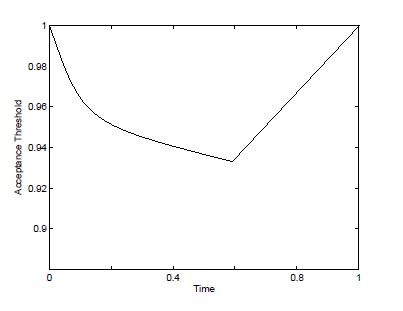
\includegraphics[width=0.5\textwidth]{ell}
	\label{2}
\end{figure}

An acceptance condition is a function of the history of the previous negotiations, the current acceptance threshold, and the outcome of the negotiation at time $t$. The agent will accept a proposal $\pi$ if it receives utility bigger than his current threshold, or his next-bid to propose utility. However this classic approach is not flexible enough when dealing with a strong opponent. An agent to be able to accept reasonable $\pi$ also need to be willing to concede more, then necessary. To do so agent needs to take into account its opponent's behavior, namely, identify how actively is an opponent bidding in order to reach an agreement. For this purpose method \texttt{countUniqueBidsAtPeriod()} was introduced. It is to calculate a number of unique bids within a given time frame. The method's pseudo-code is shown below.
\begin{verbatim}
countUniqueBidsAtPeriod(double t1, double t2) {
    if (getOpponentBids().filterByTime(t1, t2).size() != 0) {
        for (bidInPeriod : bidsInPeriod) {
            ub.add(bid);
        }
        ub.removeDuplicates();
        return ub.size();
    }
    return 0;
}
\end{verbatim}
A resulting number of bids is used as a definition of $\sigma^t$ in equation~\ref{3}.

Finally define $\omega$ in equation~\ref{3}. It's purpose is in weighting the effect of $\sigma^t$ on $\lambda$, dependent on the behavior of the opponent. In this work $\omega$ was calculated as:
\begin{dmath} \label{6}	
	\omega = \frac{getUniqueBidsCount()}{getOpponentBidHistory().size()},
\end{dmath}
where divider is received from the Bidding Strategy class. Therefore $\omega$ controls a decrease of the $\lambda$ and of the acceptance threshold as a consequence.

In addition to the described above threshold a \textit{"pressure"} threshold was defined. It was found as shown:
\begin{dmath} \label{7}	
	pressureThreshold = onbu\cdot(1 - p)\cdot e^{1 - onbu},
\end{dmath}
where $onbu$ - is an opponent next bid's utility received from the Opponent Model class, and $p$ - a user specified pressure constant in a range $(0\dots1)$.

Lastly the agent's Acceptance Strategy is comprised of the following statement represented in pseudo-code below:
\begin{verbatim}
if(lastOpponentBidUtil <= weakThreshold * \delta) {
    Reject();
}
if(lastOpponentBidUtil >= acceptanceThreshold
    or lastOpponentBidUtil >= pressureThreshold) {
    Accept();
}
Reject();
\end{verbatim}
Here \texttt{weakThreshold} is provided by the Opponent Model, which is described in the next section.

\section{Opponent Model}  

An opponent model is based on the Hard-Headed Opponent Model of the Genius-BOA framework.

Besides from the basic model, there are two extra components .~\cite{anac2013}

\subsection{Simple Frequency}

The Simple frequency model only updates weights when the bid change often.
That means that the weights of the model are only changed when the opponents bids pass a certain numerical threshold.

\subsection{Distance of the opponent}

The opponent model also calculates a threshold that is used in the Acceptance Strategy and is based on the distance of the opponent.

\textbf{ The basic algorithm of the distance of the opponent is:}

\begin{verbatim}
	BidHistory bH            = negotiationSession.getOpponentBidHistory();
	double oponentFirstUtil  = bH.getLastBidDetails().getMyUndiscountedUtil();
    myUtility = negotiationSession.getOwnBidHistory().getLastBidDetails().getMyUndiscountedUtil();
	    
	    double dous              = myUtility - oponentFirstUtil; 
	    double NegotiatedTooLong = negotiationSession.getDiscountFactor();
	    double threshold         = 1;    
	    int horizon              = 20;    
	     double mean = calculateMean(horizon);
	     double variance  = calculateVariance(horizon,mean);
	     double time = negotiationSession.getTime();
	     threshold = (mean +dous) / 2;
	     if(time > .8){
	        	if(time > .9) threshold += (1 - (time - 0.9)) * variance;
	        	else          threshold -= (1 - (time - 0.8)) * variance;
	     }
	     else
	         threshold += variance;
	     if(time > NegotiatedTooLong)
	         return 0;
	    return threshold;
\end{verbatim}

The \texttt{horizon} parameter, defines the number of past bids the agend takes into account when calculating the DOUS distance. The smaller the horizon, the more short-sighted the agent will be. Usually, a \texttt{horizon} set to 20 captures the fluctuations of the opponents bids efficiently.
 A parameter \textbf{NegotiatedTooLong} is introduced, and is set equal to the discount factor. That means that whenever the discount is a small number, the threshold will be kept for a small amount of time, whereas if the discount is a big number, the threshold will be kept for a bigger amount of time.
\\* The DOUS value is versatile, as it is not domain dependent.
As it is presented here, it can be implemented only on negotiations of two agents, but it can be expanded to multiple agent negotiations creating a DOUS distance for every opposing agent.The threshold that is outputted is a \texttt{weakThreshold}. That is, if the value of a bid an agent offers to the Nego Agent is smaller than the \texttt{weakThreshold}, the bid is rejected. If the value is higher, we compare it with the normal threshold computed in the Acceptance Strategy.This ensures that the agents will reject points that are far from the Nash equilibrium.
\\*The amount of time this threshold holds,is dependent on the discount factor of the negotiation. This restriction is set because the agent needs to be more concessive as the negotiation approaches the deadline. If the discount factor is 1, and no depreciation exists, this threshold stands for the whole negotiation. 
The visualization of the DOUS distance would be:

\begin{figure}[htbp]
  \caption{The distance between the initial utilities of the agents}
  \centering
    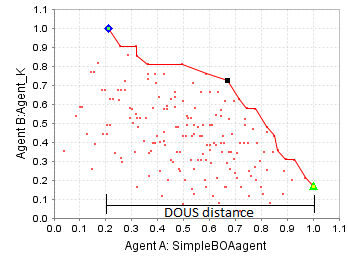
\includegraphics[width=0.5\textwidth]{dous}
    \label{3}
\end{figure}

\section{Opponent Model Strategy}  

This module was adapted from a Best Bid Strategy, included in \textit{Genius}. The idea behind it is in keeping a small history of opponent's bids for determination of the best bid. An experimentation with a history size showed that keeping of the considerable amount of opponent's bids has a negative impact on the agent's performance, thus the history size was set to $10$ independent of the domain.

The most basic OMS was selected to show the strengths and weaknesses of the NegoAgent in it's current state regardless or other variables introduced by more advanced models. However it is likely that a more tuned model is to increase the agent's performance, and thus this leaves a space for further investigation.

\section{Binding the Modules}

It is useful to have a single-entity agent instead of several BOA components. In particular, \textit{Genius} allows single-entity agents run separate sessions against each other, and \textit{ANAC} competition uses this kind of agents in the tournament series. A single-entity agent may consist of numerous parts, however the one described in the paper is comprised of four main BOA components:
\begin{itemize}
	\item Bidding Strategy
	\item Acceptance Strategy
	\item Opponent Model
	\item Opponent Model Strategy
\end{itemize}

In order to bind all the modules together, a class that extended the BOA agent and passes each of the modules with it's parameters as parts of the agent should be created. Then it is necessary to override an \texttt{agentSetup()} method of the class. The pseudo-code of the overriden class is:

\begin{verbatim}
NegoAgent extends BOAagent {    
    @Override
    agentSetup(){
        OpponentModel om = new OpponentsModel(negotiationSession);
        OMStrategy oms = new BidStrategy(negotiationSession , om);
        OfferingStrategy offering = new NegoAgent_TDOffering(nego-
        tiationSession, om, oms, Pmax, Pmin);
        AcceptanceStrategy ac =  new AStrategy(negotiationSession,
        offering, a , b, c);
        setDecoupledComponents (ac, offering, om, oms );
    }
}
\end{verbatim}

\section{Results}

The agent implemented is a very-strong willed agent. It accepts bids faster when the discount factor is big, otherwise it negotiates longer. An Acceptance Strategy with the weak threshold enables it to accept offers that are at least close to Nash equilibrium, when  $t\to1$, therefore it accepts more reasonable bids. Its TD offering makes the agent extremely efficient at obtaining the best utility possible from strong willed opponents. The figures below show the results against a very good 2013 agent.

\begin{table}[ht] 

\centering % used for centering table 
\caption{Results of agent negotiations} % title of Table 
\begin{tabular}{ccccccccc} % centered columns
\hline\hline %inserts double horizontal lines 
 Opponent & A  &  B & Rounds & u A & u B & $\delta$u A & $\delta$u B & $t$\\ [0.5ex] % inserts table 
\hline
%heading 
\hline % inserts single horizontal line 
Meta&Cypress&Itex&6517&0.9268&0.3073&0.9268&0.3073&0.9822\\
Meta&Itex&Cypress&7475&0&0&0&0&1\\
Simple&Sam&Mary&41&1&0.4500&0.9755&0.4390&0.1148\\
Simple&Mary&Sam&73&1&0.5250&0.9591&0.5035&0.1932\\ 
TitforTat&CarA1&CarA2&1406&0.9641&0.8936&0.7269&0.6737&0.9818\\
TitforTat&CarA2&CarA1&1536&0.9800&0.7642&0.7360&0.5739&0.9953\\
Negotiator&SmartPhone1&SmartPhone2&1145&0.9585&0.6635&0.8466&0.5861&0.8911\\
Negotiator&SmartPhone2&SmartPhone1&1061&0.9776&0.5540&0.8605&0.4877&0.9158\\
CUHKA&NiceOrDie1&NiceOrDie2&3681&0.2990&0.2990&0.2243&0.2243&0.9990\\
CUHKA&NiceOrDie2&NiceOrDie1&3437&0.2990&0.2990&0.2243&0.2243&0.9986\\
[1ex] % [1ex] adds vertical
\hline %inserts single line 
\end{tabular} 
\caption{u X: utility of agent X , $\delta$u X:discounted utility of agent X} % title of Table 
\label{table:NegoSimpleresults} % is used to refer this table in the text 
\end{table} 

\section{Conclusion and further work}
Building a negotiating agent is a non-trivial matter, as the negotiation domains are practically infinite, as are the strategies that can be used. As the agent negotiation is a research field that has only been introduced recently, and as there are strategies that behave well given different domains there is a lot of research to be done, until we reach a universal strategy, or a strategy that works very well in all of the domains.

\begin{thebibliography}{}

\bibitem{abines} 
Hao J., Leung H.:
ABiNeS: An Adaptive Bilateral Negotiating Strategy over Multiple Items

\bibitem{genius}
Genius platform at TU Delft,
\texttt{http://www.mmi.tudelft.nl/genius/} Retrieval date: 01.12.13

\bibitem{anac2013}
Something

\end{thebibliography}

\end{document}